\myparagraph{Purpose}
Anyone who wants to subscribe to one or both services offered by \textit{Data4Help} must go through the registration process, which can be carried out either through \textit{AutomatedSos} and \textit{Track4Run} apps or through the web site.
The process requires exactly the same steps regardless the platform through which it is carried out:
\begin{enumerate}
  \item The new user is required to fill in all the fields in which he/she is asked for his/her name, his/her surname, his/her date of birth, his/her city of birth, his/her city of residence, his/her address, his/her occupation, and a valid e-mail address;
  \item The user must accept the conditions regarding his/her privacy, in particular about the collection of his/her data by \textit{Data4Help} and the sharing of them in anonymous way with third parties.
\end{enumerate}
After that the system will check the correctness of the inserted data, in particular it will check that the user isn't already registerd and that the inserted e-mail isn't already used by someone else. If the result of this control is positive the registration is authorized and the user will receive a confermation e-mail to the specified e-mail address with the password he/she has to use to access to all \textit{Data4Help} services.

\myparagraph{Scenario 1} \label{aSOSsignin}
Sara would like to register her grandmother to \textit{AutomatedSos} to not worry about her helth status when they are not together. She opens the browser on her personal computer and search for \textit{Data4Help} web site, then she clicks on the "\textit{Sign In}" button, which is located in the main page. She passes through the steps of the registration process, inserting her grandmother data and accepting the required conditions. Finally, if the inserted data are accepted by the system, she receives the confirmation e-mail.

\myparagraph{Scenario 2}
Marco wuold like to organize an amateur run with his friends and remembers that someone told him something about a new application called \textit{Track4Run} so he decides to try it. He downloads the app on his smartphone and turns it on. The first page that is shown to him contains the "\textit{Sign In}" button and the "\textit{Log In}" one, he presses on the first one and starts his registration process. He doesn't use his personal e-mail address, but an e-mail address he has in common with his brother that they usually use to make purchase online. Unexpectedly he is informed by the system that the insert e-mail is already registered in the database and so he has to change it and this time he inserts his personal e-mail address. This time the registration is succesfull and he receives the confermation e-mail.

\myparagraph{Use Case}
The \textit{Individual Sign In} use case is analyzed in Table \ref{table:individualSignInTable}.

\myparagraph{Mockup}
The \textit{Individual Sign In} mocukp is shown in Figure \ref{img:individualSignInMockup}.

\myparagraph{Functional requirements}
\begin{enumerate}
  \item The system must not accept an e-mail address that is already used by an already registered user;
  \item The system must not authorize the registration untill all the fields are filled up;
  \item The system must not authorize the registration untill the required conditions aren't accepted;
  \item The system must send the confirmation e-mail to the inserted e-mail address with the password when "\textit{Submit}" button is clicked only if all the inserted data are acceptable and the required conditions has been accepted;
  \item The system must let the \textbf{Individual user to be} leave the registration process at anytime.
\end{enumerate}

\clearpage
\thispagestyle{empty}
\begin{center}
\begin{table}
\begin{tabular}{ | l | p{0.75\linewidth} | }
  \hline
    Actor & \textbf{Individual user to be} \\ \hline
    Goal & \textbf{[G.1]} \\ \hline
    Input Condition & A person wants to subscribe to one of \textit{Data4Help} services \\ \hline
    Event Flow & \begin{minipage}[t]{0.7\textwidth}
      \begin{enumerate}
        \item The \textbf{Individual user to be} opens the main page of \textit{Data4Help} web site from his/her personal computer or of \textit{AutomatedSos} or \textit{Track4Run} apps from his smartphone;
        \item The \textbf{Individual user to be} clicks on the "\textit{Sign in}" button;
        \item The system shows the form the \textbf{Individual user to be} has to fill up;
        \item The \textbf{Individual user to be} fills up the form with his/her name, his/her surname, his/her date of birth, his/her city of birth, his/her city of residence, his/her address, his/her occupation, and a valid e-mail address;
        \item The \textbf{Individual user to be} accepts the required conditions;
        \item The \textbf{Individual user to be} clicks on the "\textit{Submit}" button;
        \item The system checks wheter the inserted information are acceptable or not;
        \item The \textbf{Individual user to be} receives a confirmation e-mail containing the password he/she has to use to access to all \textit{Data4Help} services.
      \end{enumerate}
    \smallskip
  \end{minipage} \\ \hline
  Output Condition & The system tells the \textbf{Individual user to be} that his/her registration is completed \\ \hline
  Exceptions & \begin{minipage}[t]{0.7\textwidth}
    \begin{itemize}
      \smallskip
      \item If functional requirements 1 or 2 are not satisfied the process goes back to step 4;
      \item If functional requirement 3 is not satisfied the process goes back to step 5;
      \item If the \textbf{Individual user to be} decides to leave the registration process this one is aborted.
    \end{itemize}
    \smallskip
  \end{minipage}  \\ \hline
\end{tabular}
\caption{\textit{Individual Sign In} use case}
\label{table:individualSignInTable}
\end{table}
\end{center}
\clearpage

\begin{figure}
\begin{center}
  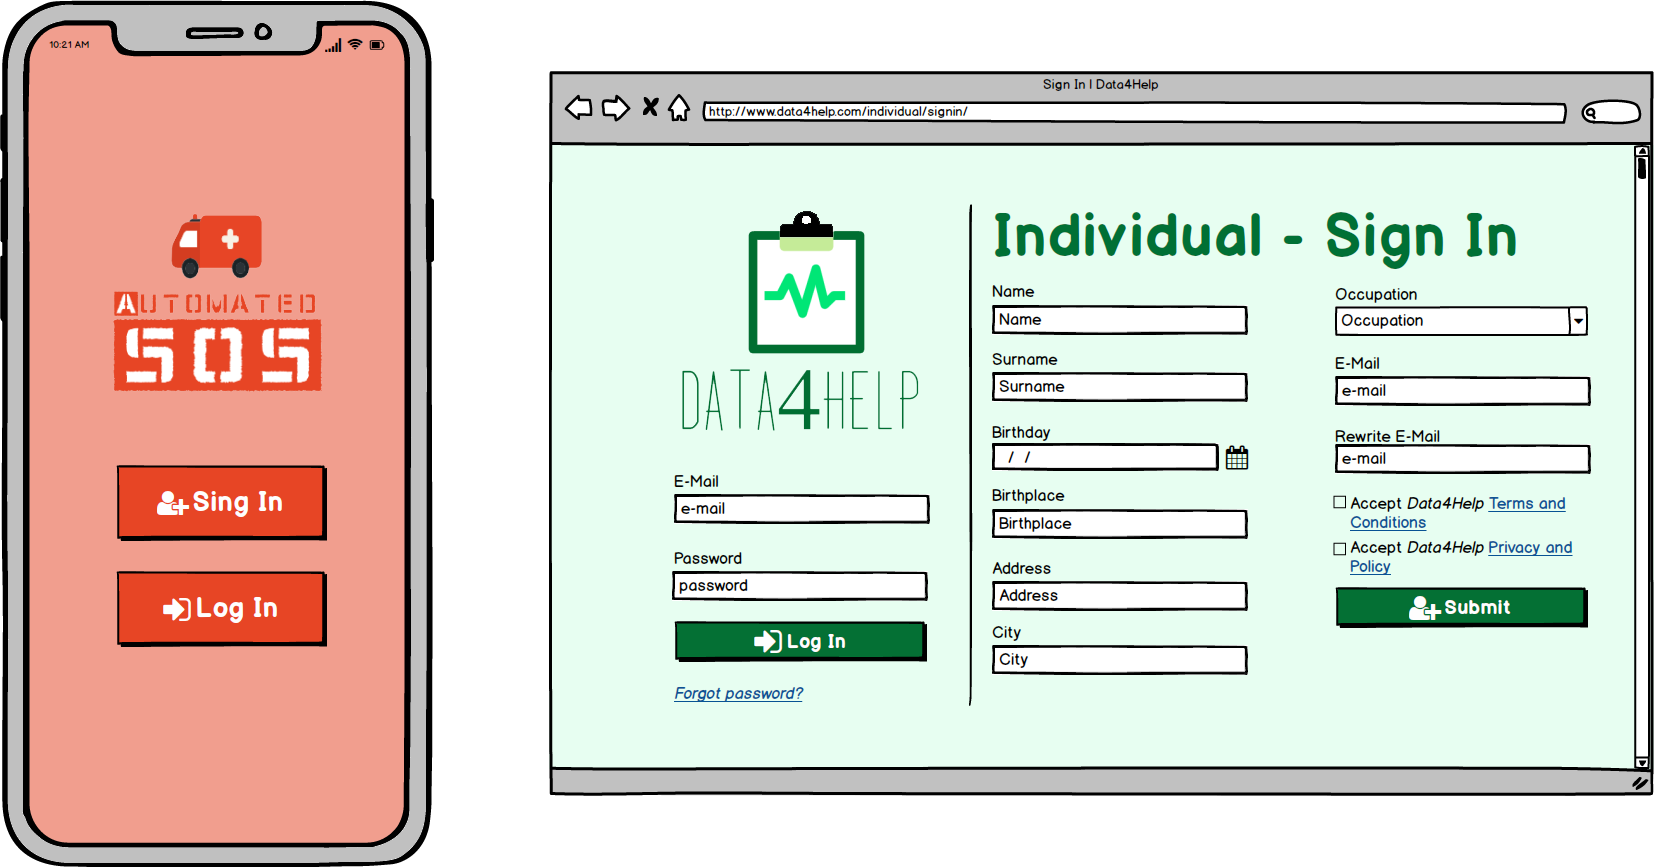
\includegraphics[width=\textwidth]{img/mockup/Individual_SingIn.png}
  \hspace{0.05\linewidth}
  \centering
  \caption{\textit{Individual Sign In} mockup}
  \label{img:individualSignInMockup}
\end{center}
\end{figure}
